\documentclass{beamer}
\usepackage[utf8]{inputenc}
\usetheme{Madrid}
\usecolortheme{default}
\usepackage{amsmath,amssymb,amsfonts,amsthm}
\usepackage{txfonts}
\usepackage{tkz-euclide}
\usepackage{listings}
\usepackage{adjustbox}
\usepackage{array}
\usepackage{tabularx}
\usepackage{gvv}
\usepackage{lmodern}
\usepackage{circuitikz}
\usepackage{tikz}
\usepackage{graphicx}

\setbeamertemplate{page number in head/foot}[totalframenumber]

\usepackage{tcolorbox}
\tcbuselibrary{minted,breakable,xparse,skins}



\definecolor{bg}{gray}{0.95}
\DeclareTCBListing{mintedbox}{O{}m!O{}}{%
  breakable=true,
  listing engine=minted,
  listing only,
  minted language=#2,
  minted style=default,
  minted options={%
    linenos,
    gobble=0,
    breaklines=true,
    breakafter=,,
    fontsize=\small,
    numbersep=8pt,
    #1},
  boxsep=0pt,
  left skip=0pt,
  right skip=0pt,
  left=25pt,
  right=0pt,
  top=3pt,
  bottom=3pt,
  arc=5pt,
  leftrule=0pt,
  rightrule=0pt,
  bottomrule=2pt,
  toprule=2pt,
  colback=bg,
  colframe=orange!70,
  enhanced,
  overlay={%
    \begin{tcbclipinterior}
    \fill[orange!20!white] (frame.south west) rectangle ([xshift=20pt]frame.north west);
    \end{tcbclipinterior}},
  #3,
}
\lstset{
    language=C,
    basicstyle=\ttfamily\small,
    keywordstyle=\color{blue},
    stringstyle=\color{orange},
    commentstyle=\color{green!60!black},
    numbers=left,
    numberstyle=\tiny\color{gray},
    breaklines=true,
    showstringspaces=false,
}
%------------------------------------------------------------
%This block of code defines the information to appear in the
%Title page
\title %optional
{2.2.30}

%\subtitle{A short story}

\author % (optional)
{stalin-ai25btech11026}



\begin{document}


\frame{\titlepage}
\begin{frame}{Question}
 Find the angle between the line 
\begin{align}
\frac{x+1}{2} = \frac{y}{3} = \frac{z-3}{6}
\end{align}
and the plane 
\begin{align}
10x + 2y - 11z = 3.
\end{align}

.\\ 
\end{frame}
\begin{frame}{Theoretical Solution}
Let us solve the given equation theoretically and then verify the solution computationally \\
According to the question, \\
Given a plane and line\\
Let $\theta$ be angle between plane and line\\
Then $90^\circ-\theta$ is angle between normal vector of plane and line\\
Let $\vec{D}$ be dirction vector of line and $\vec{n}$ be normal of plane\\
\begin{align}
\vec{D}=\begin{myvec}{2\\3\\6}\end{myvec}\
\vec{n}=\begin{myvec}{10\\2\\-11}\end{myvec}\
\end{align}
\begin{align}
   \cos(90^\circ-\theta)=\frac{\vec{D}^T\vec{n}}{\|\vec{n}\|\|\vec{D}\|}=\frac{-8}{21}
\end{align}


\end{frame}
\begin{frame}{Theoretical Solution}
\begin{align}
    \theta=90^\circ-\cos^{-1} (\frac{-8}{21})=-22.39^\circ
\end{align}
angle is $22.39^\circ$
\end{frame}
\begin{frame}[fragile]
    \frametitle{C Code}
    \begin{lstlisting}
#include <stdio.h>
#include <math.h>

int main() {
    // Direction ratios of the line
    double dx = 2, dy = 3, dz = 6;
    
    // Normal vector of the plane
    double nx = 10, ny = 2, nz = -11;
    
    // Dot product of d and n
    double dot = dx * nx + dy * ny + dz * nz;
    
    // Magnitudes of d and n
    double mag_d = sqrt(dx*dx + dy*dy + dz*dz);
    double mag_n = sqrt(nx*nx + ny*ny + nz*nz);
    
    // Calculate the cosine of angle phi between d and n
    double cos_phi = fabs(dot) / (mag_d * mag_n);
    
    

     \end{lstlisting}
\end{frame}
\begin{frame}[fragile]
    \frametitle{C Code }
    \begin{lstlisting}
     // Calculate phi in radians
    double phi = acos(cos_phi);
    
    // Angle between line and plane
    double theta = (M_PI / 2) - phi;
    
    // Convert to degrees
    double angle_degrees = theta * (180.0 / M_PI);
    
    printf("The angle between the line and the plane is: %.2f degrees\n", angle_degrees);
    
    return 0;
}
\end{lstlisting}
\end{frame}
\begin{frame}[fragile]
    \frametitle{python code }
    \begin{lstlisting}
   import numpy as np
import matplotlib.pyplot as plt
from mpl_toolkits.mplot3d import Axes3D

# Line: (x+1)/2 = y/3 = (z-3)/6
# Direction ratios of line
d = np.array([2, 3, 6])

# Plane: 10x + 2y - 11z = 3
n = np.array([10, 2, -11])  # normal vector of plane

# Angle between line and plane
# angle θ = 90° - angle(line, normal)
cos_theta = abs(np.dot(d, n)) / (np.linalg.norm(d) * np.linalg.norm(n))
theta = np.arcsin(cos_theta)  # angle between line and plane in radians
theta_deg = np.degrees(theta)
    \end{lstlisting}
\end{frame}
\begin{frame}[fragile]
    \frametitle{python code }
    \begin{lstlisting}
print("Angle between line and plane = ", theta_deg, "degrees")

# ---------- Plotting ----------
fig = plt.figure()
ax = fig.add_subplot(111, projection='3d')

# Create grid for plane
xx, yy = np.meshgrid(range(-5, 6), range(-5, 6))
zz = (10*xx + 2*yy - 3) / 11  # from plane equation

# Plot plane
ax.plot_surface(xx, yy, zz, alpha=0.5, color='cyan')

# Line parametric form: x = -1 + 2t, y = 3t, z = 3 + 6t
t = np.linspace(-2, 2, 50)
x_line = -1 + 2*t
y_line = 3*t
z_line = 3 + 6*t

\end{lstlisting}
\end{frame}
\begin{frame}[fragile]
    \frametitle{python code }
    \begin{lstlisting}
# Plot line
ax.plot(x_line, y_line, z_line, color='red', linewidth=2, label="Line")

# Formatting
ax.set_xlabel('X')
ax.set_ylabel('Y')
ax.set_zlabel('Z')
ax.set_title(f"Angle = {theta_deg:.2f}°")
ax.legend()

# Save the figure
plt.savefig("line_plane_angle.png", dpi=300)
plt.show()
    \end{lstlisting}
\end{frame}
\begin{frame}{Plot}
    \centering
    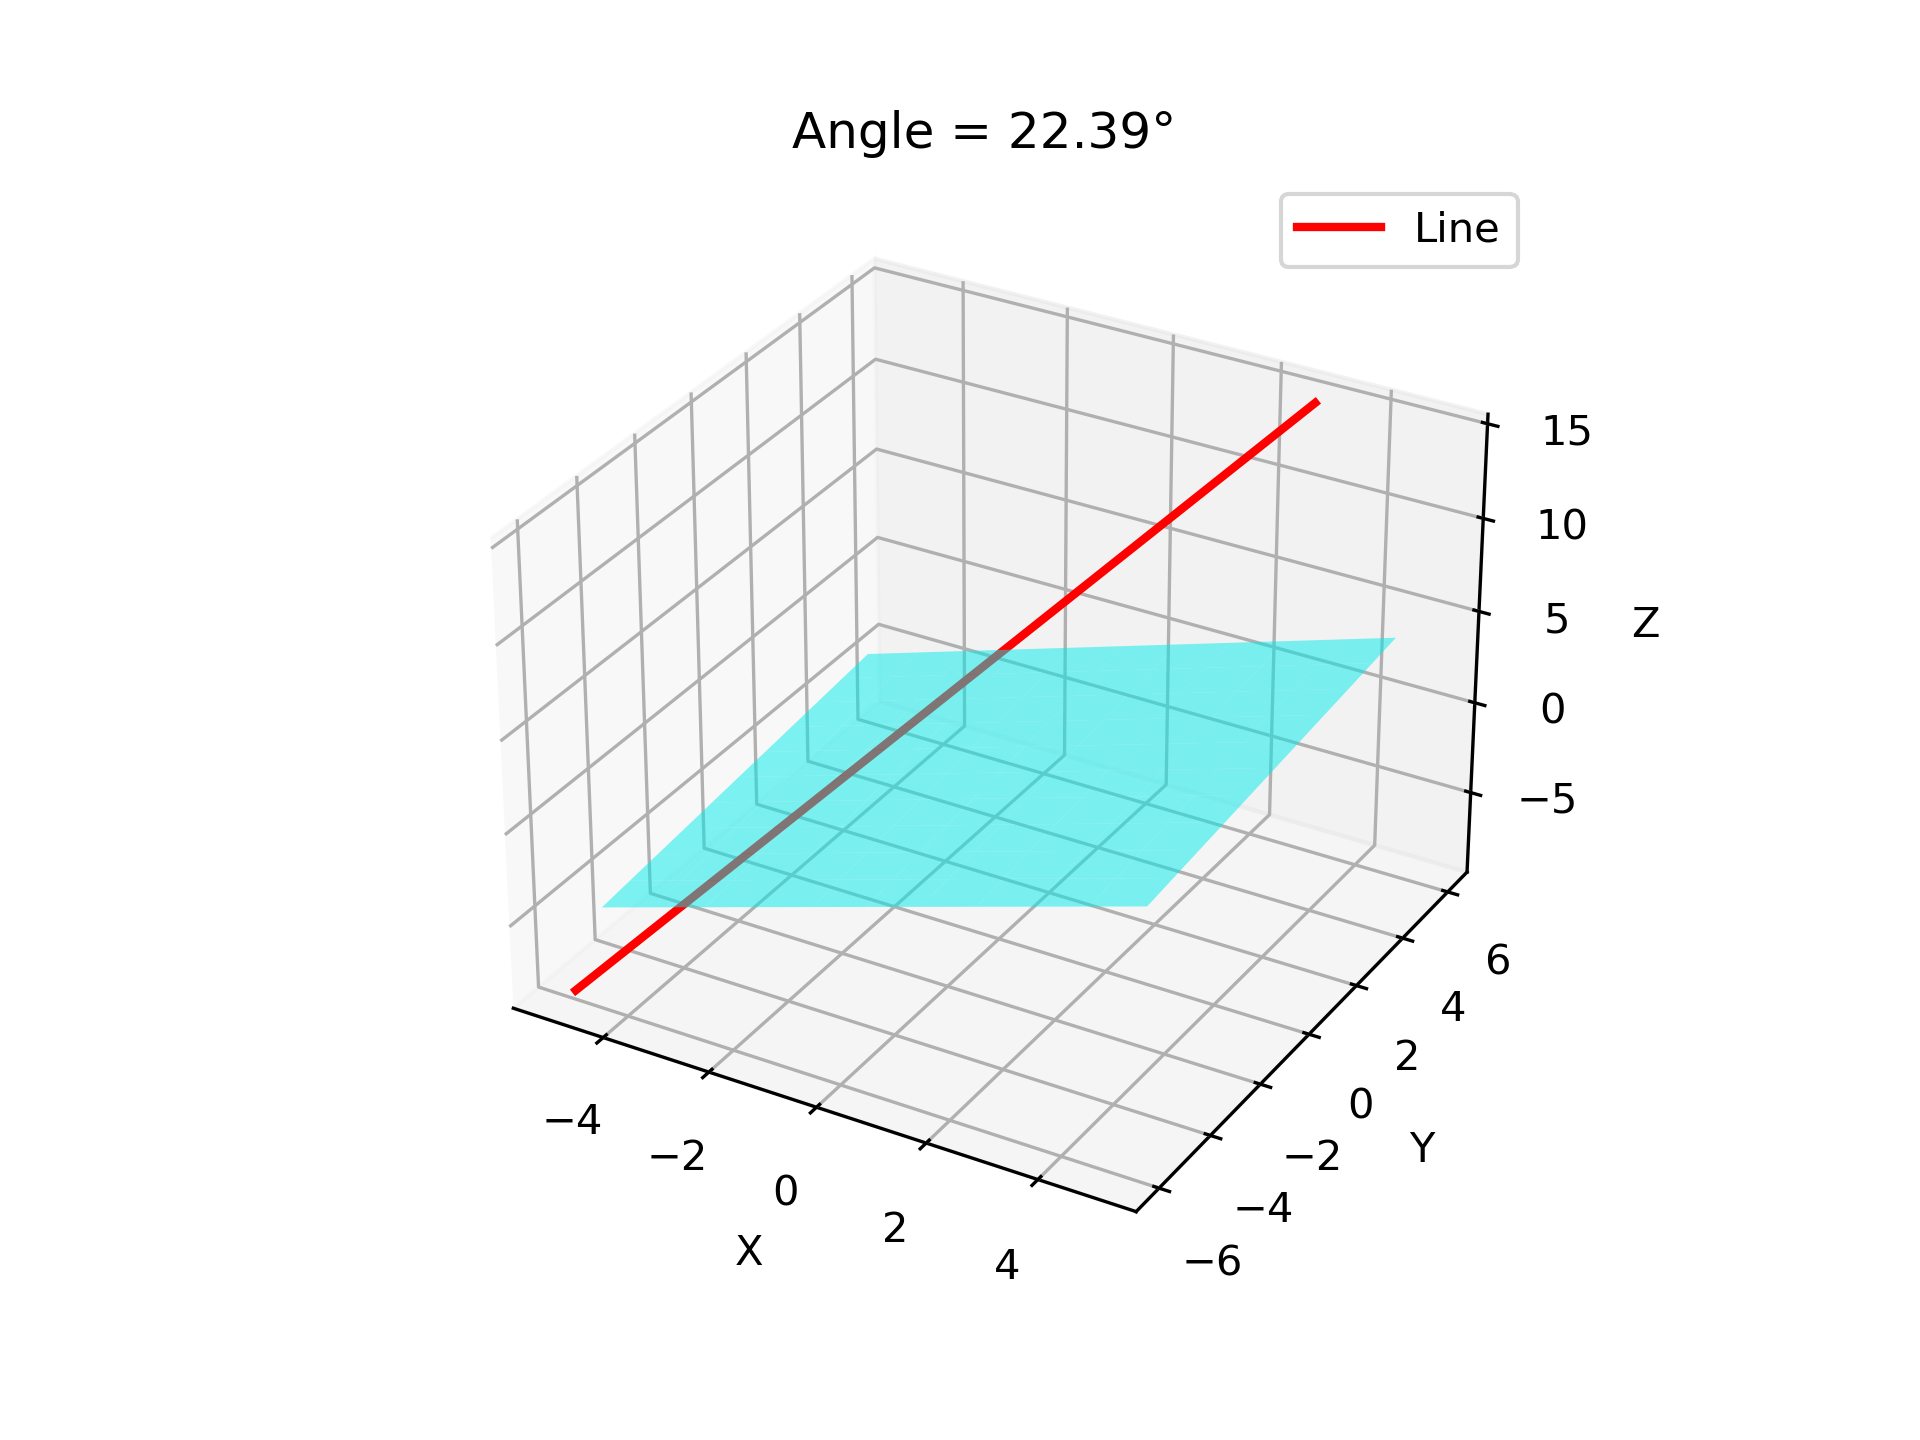
\includegraphics[width=\columnwidth, height=0.8\textheight, keepaspectratio]{figs/line_plane_angle.png}     
\end{frame}

\end{document}